\documentclass[pdf,10pt]{beamer}
\usepackage{latexsym,amssymb,amsmath,amsbsy,amsopn,amstext,xcolor,multicol}
\usepackage{graphicx,wrapfig,fancybox}
\usepackage{pgf,pgfarrows,pgfnodes,pgfautomata,pgfheaps,pgfshade}
\usepackage{booktabs}      %有加粗的三线表格
\usepackage[utf8]{inputenc}
\usepackage{subfloat}
\usepackage{natbib}
\usepackage{}

\usetheme{Darmstadt}
\usecolortheme{beaver}
\beamersetaveragebackground{black!2}
\graphicspath{{figures/}}  %图片路径

\bibliographystyle{apalike}
\def\newblock{}

\begin{document}

\title{The Presentation of Entities and Relations and its Application in Inference}
\subtitle{}
\author{Weidi Xu}
\institute{Peking University, Computational Intelligence Laboratory}
\date{\today}
\frame{\titlepage}


%overview
\begin{frame}
	\frametitle{Overview}
	\begin{itemize}
		\item Knowledge Graph: a directed graph with entiites and relations
		\item Knowledge Inference: link prediction in knowledge graph
		\item Representation: efficient and scalable inference methods
	\end{itemize}
\end{frame}

\begin{frame}
\frametitle{Table of Contents}
\tableofcontents
\end{frame}

\AtBeginSection[]
{
	\begin{frame}
	\frametitle{Table}
	\tableofcontents[currentsection]
	\end{frame}
}


\section{Background}

\subsection{Kowledge Graph}
\begin{frame}
\frametitle{Knowledge Graph}
\begin{itemize}
	\item Knowledge graph is a directed graph comprised by entities and relations. 

	\begin{columns}[onlytextwidth]
		\begin{column}{0.45\textwidth}
			\begin{figure}
				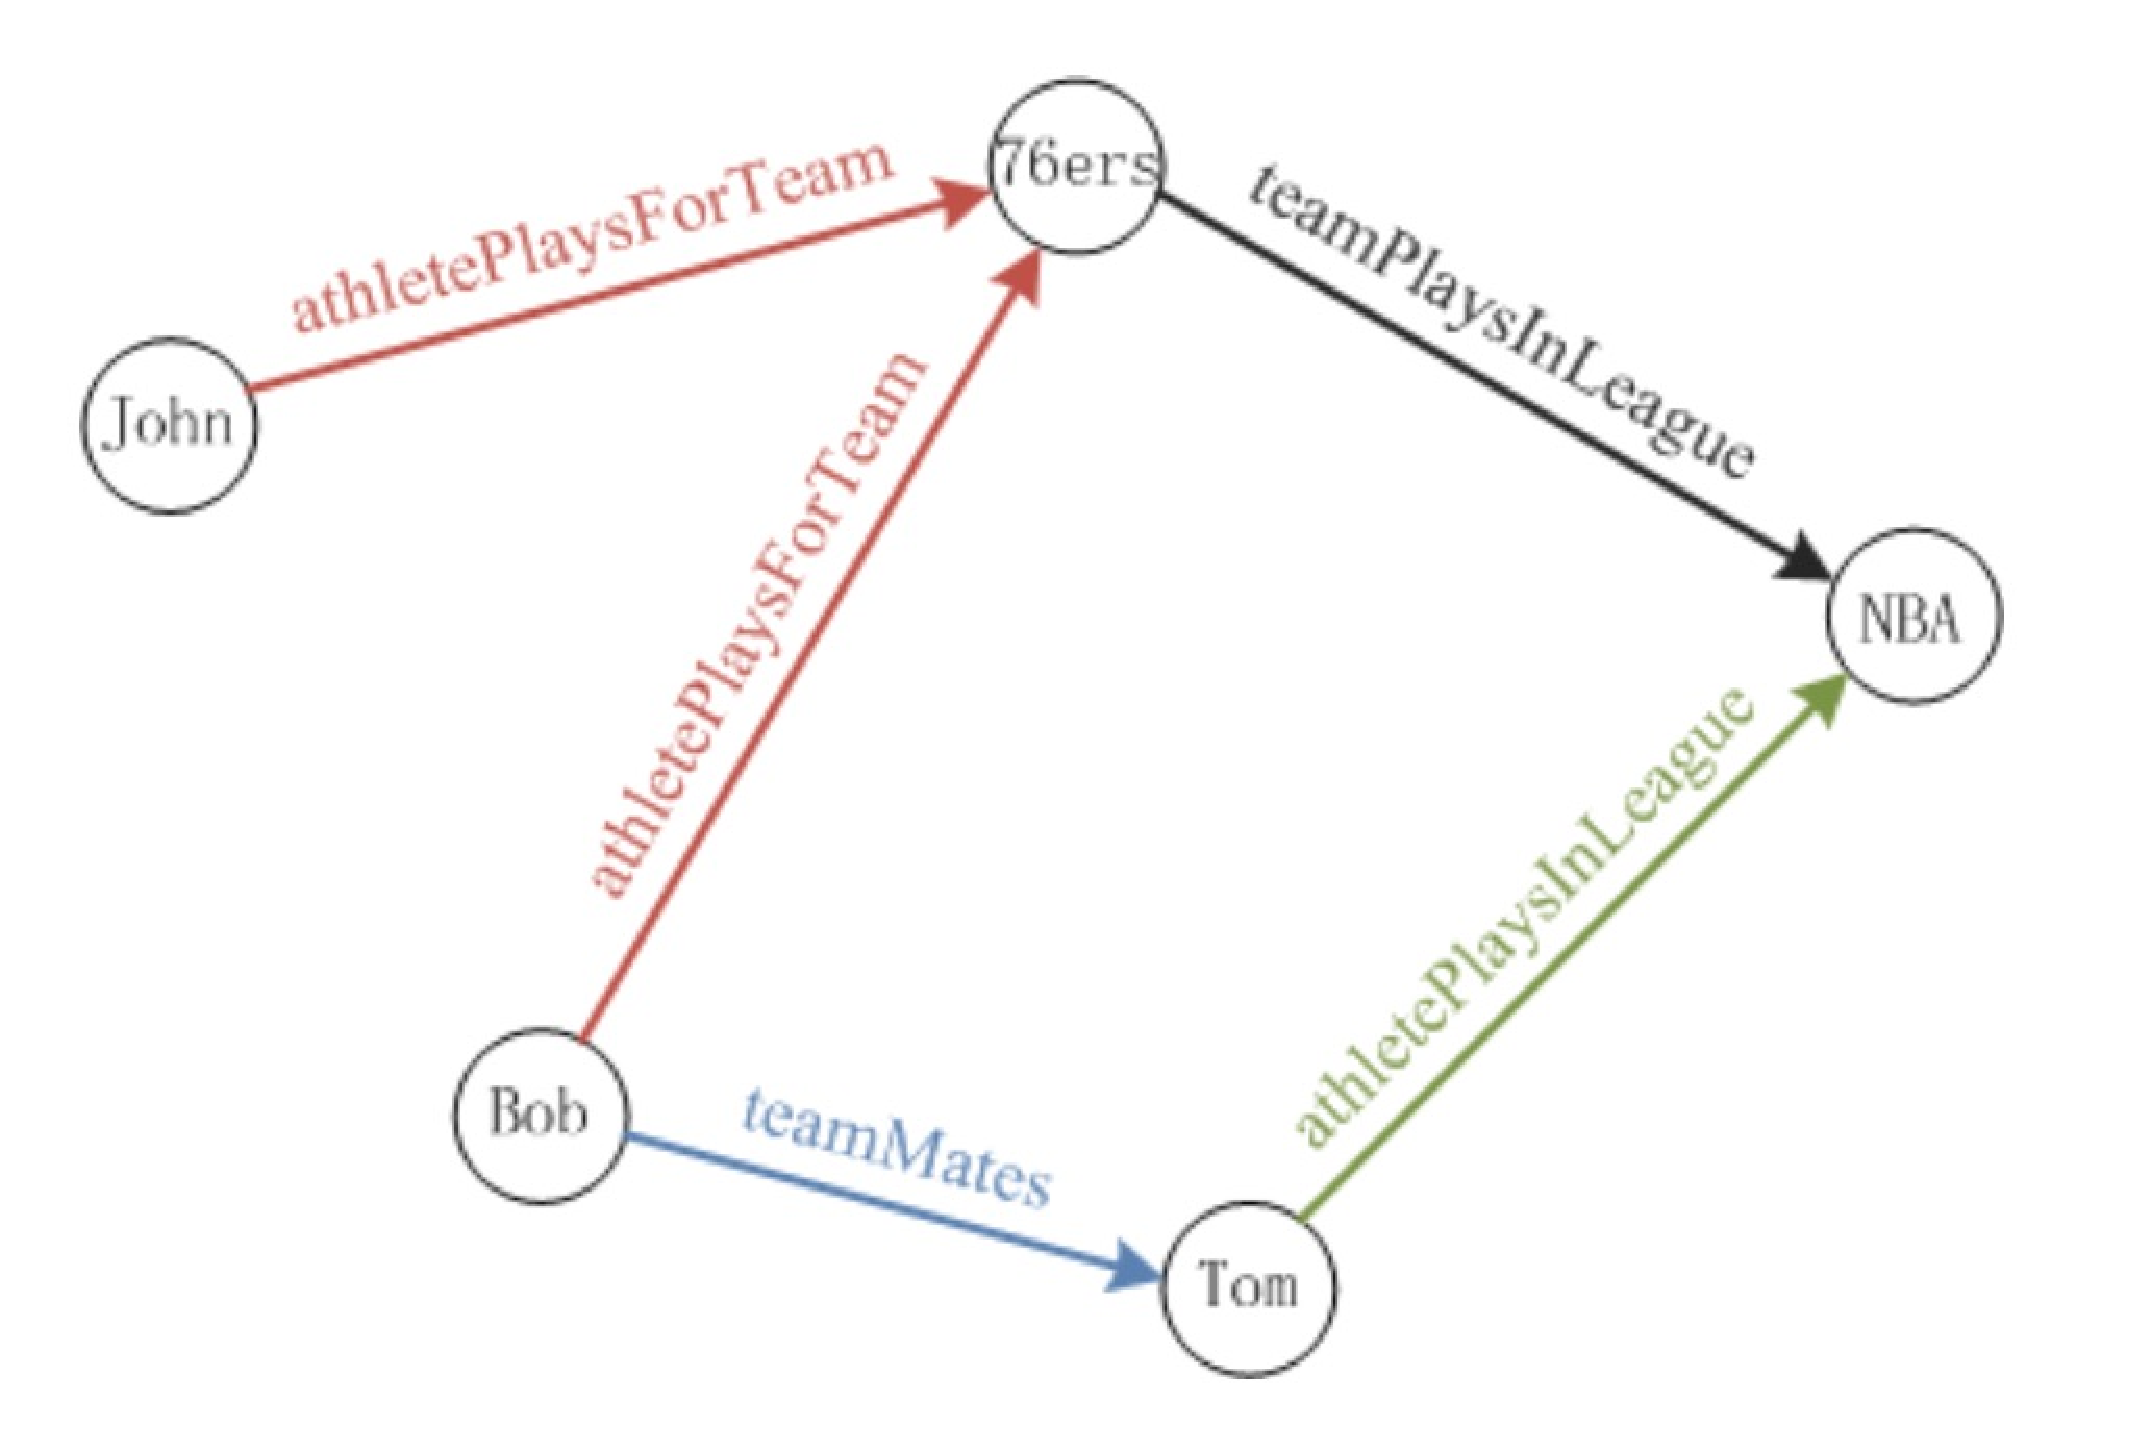
\includegraphics[width=.45\textwidth,natwidth=610,natheight=610]{2.eps}
			\end{figure}
		\end{column}
		\begin{column}{0.45\textwidth}
			\begin{itemize}
			\begin{tiny}
				\item (John, athletePlaysForTeam, 76ers)
				\item (Bob, athletePlaysForTeam, 76ers)
				\item (Tom, athleteMates, Tom)
				\item (Tom, athletePlaysInLeague, NBA)
				\item (76ers, teamPlaysInLeague, NBA)
			\end{tiny}
			\end{itemize}
		\end{column}
	\end{columns}
	\item However the knowledge graph is incomplete: it only covers small part of facts.
	\end{itemize}
\end{frame}

\subsection{Knowledge Inference}
\begin{frame}
\frametitle{Knowledge Inference}
\begin{itemize}
	\item Knowledge inference: link prediction in knowledge graph.

	\begin{columns}[onlytextwidth]
		\begin{column}{0.45\textwidth}
			\begin{figure}
				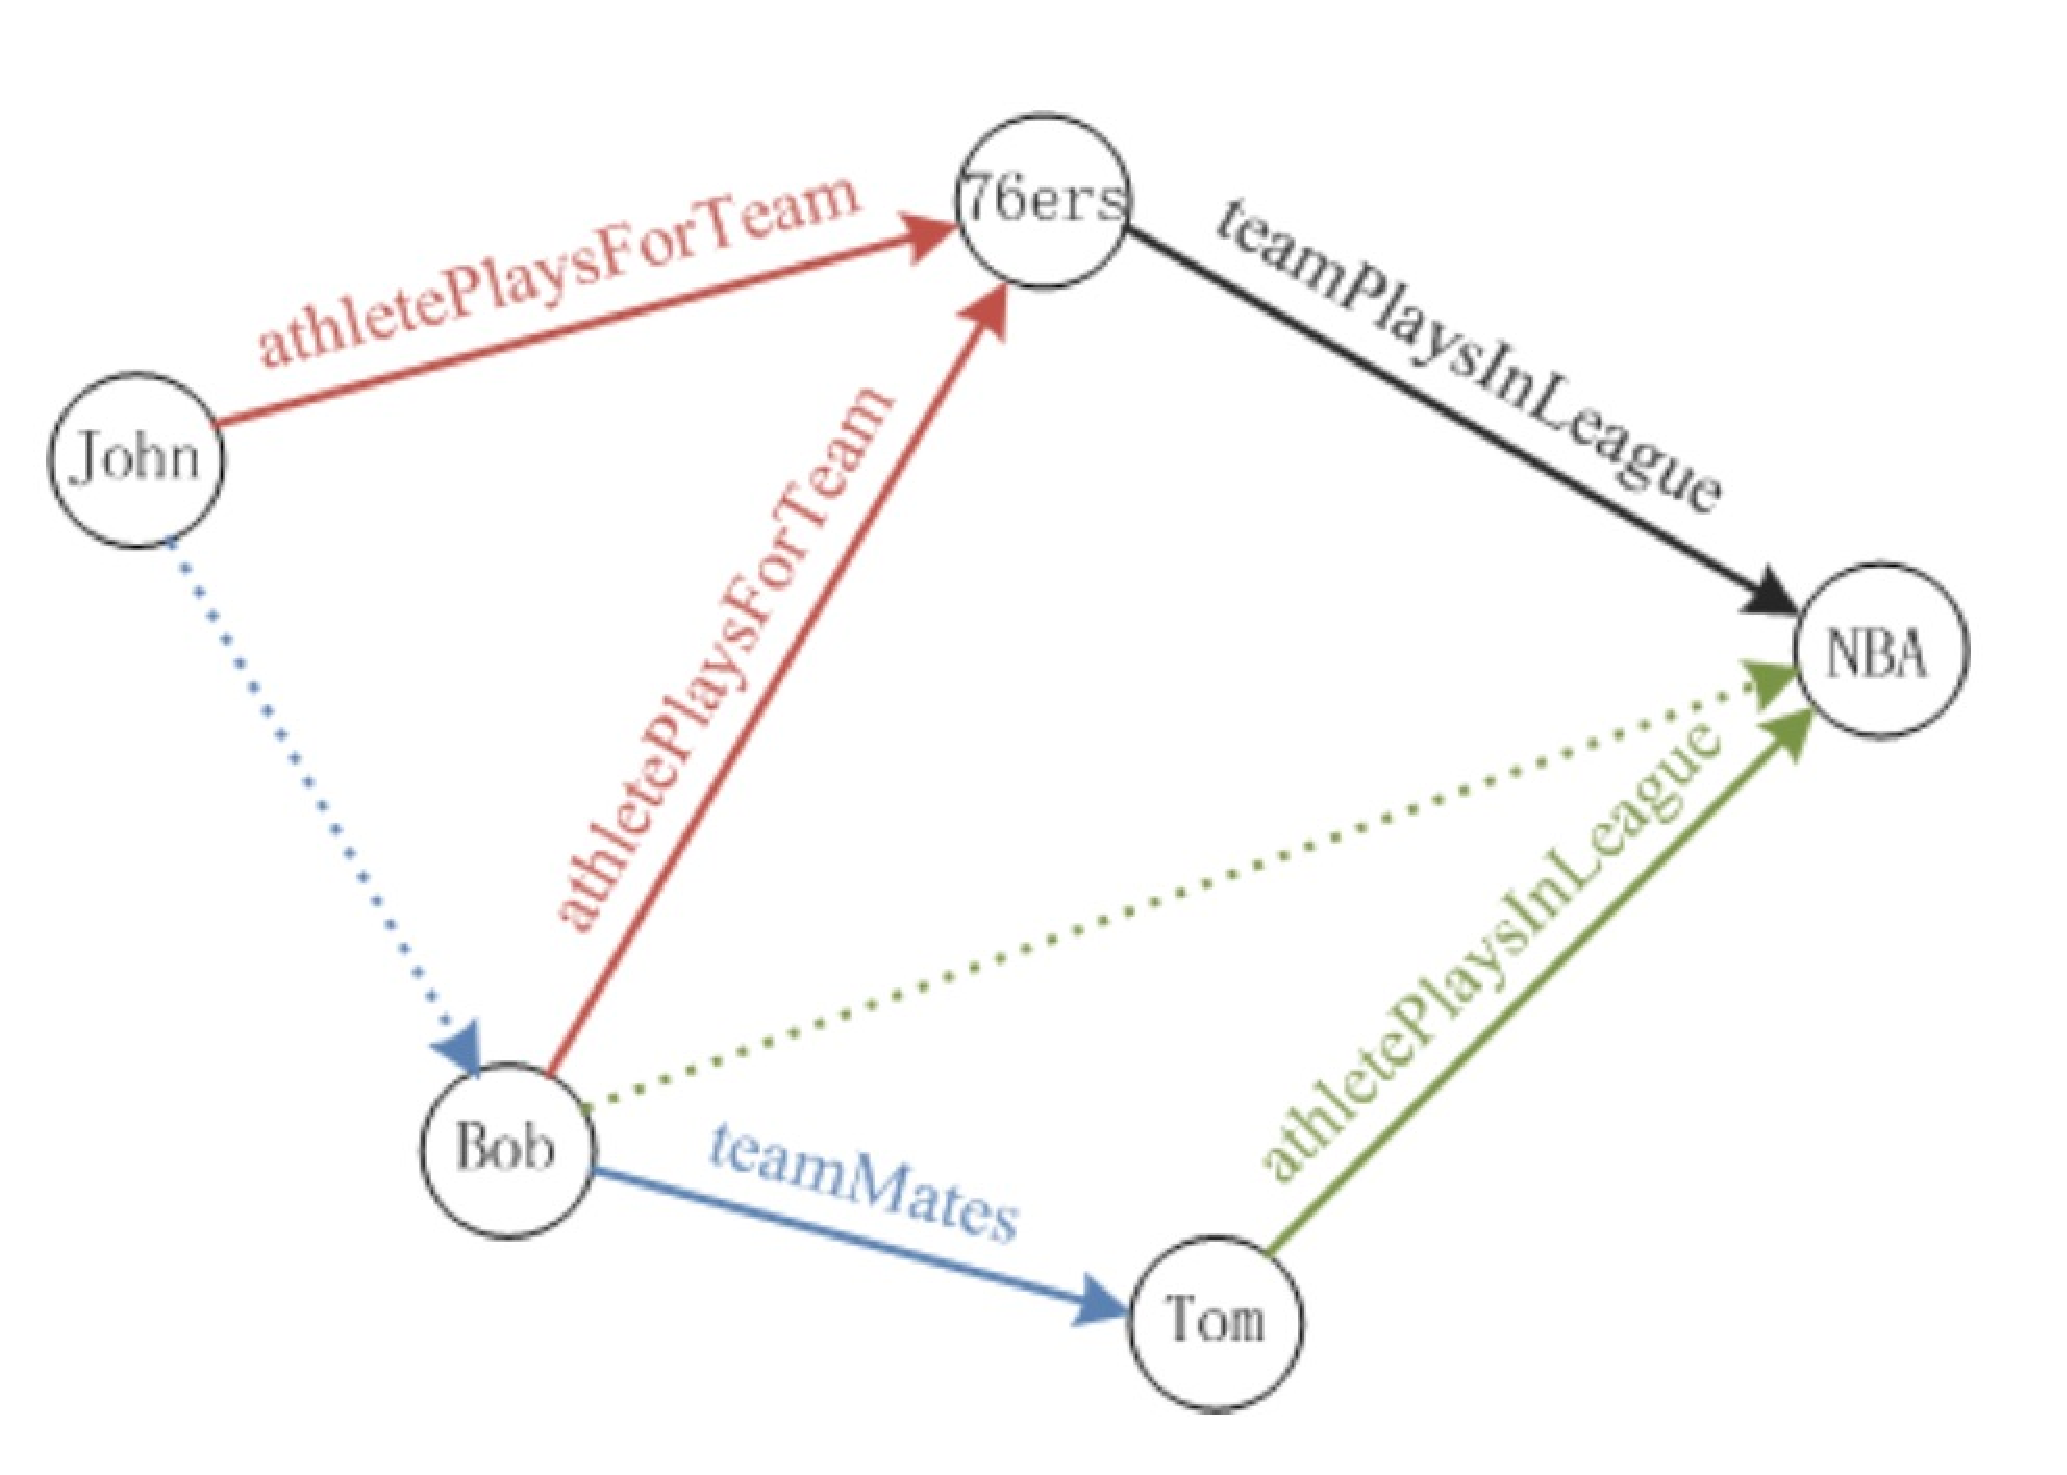
\includegraphics[width=.45\textwidth,natwidth=610,natheight=610]{4.eps}
			\end{figure}
		\end{column}
		\begin{column}{0.45\textwidth}
			\begin{itemize}
			\begin{tiny}
				\item (John, teamMates, Bob)
				\item (Bob, athletePlaysInLeague, NBA)
				\item ... ...
			\end{tiny}
			\end{itemize}
		\end{column}
	\end{columns}
	\item Inference in Knowledge Graph can increase the coverage.
\end{itemize}
\end{frame}

\subsection{Methods}
\begin{frame}
\frametitle{Methods}
\begin{itemize}
	\item Inference based on representation learning.
		\begin{enumerate}
			\item Collective Matrix Factoriation \citep{nickel2011three}
			\item Neural Tensor Networks \citep{socher2013reasoning}
			\item Translating Embeddings\citep{bordes2013translating}
		\end{enumerate}
	\item Inference based on markov random field.
		\begin{enumerate}
			\item Markov Logic Networks \citep{richardson2006markov}
			\item Probabilistic Soft Logic \citep{brocheler2012probabilistic}
		\end{enumerate}
	\item Inference based on random walk.
		\begin{enumerate}
			\item Path Ranking \citep{lao2011random}
		\end{enumerate}
\end{itemize}
\end{frame}

\section{Representation learning for knowledge graph}

\subsection{Framework}
\begin{frame}
	\frametitle{Framework}
	\begin{itemize}
		\item Hidden variable model: modeling data in hidden variable space.
	\end{itemize}
	\begin{block}{Leanring}
		\begin{itemize}
			\item Learning entity and relation embeddings in hidden vector spaces.
			\item Define an fitness funtion to determine the certainty of entity-relation-entity pairs.
			\item Define an objective funtion to determine the certainty of entity-relation-entity pairs.
		\end{itemize}
	\end{block}
	\begin{alertblock}{Prediction}
		\begin{itemize}
			\item Using the model and objective function to inference.
		\end{itemize}
	\end{alertblock}
\end{frame}

\begin{frame}
	\frametitle{Framework}
	\begin{itemize}
		\item Hidden variable model: modeling data in hidden variable space.
	\end{itemize}
	\begin{block}{Leanring}
		\begin{itemize}
			\item Learning entity and relation embeddings in hidden vector spaces.
			\item Define an fitness funtion to determine the certainty of entity-relation-entity pairs.
			\item Define an objective funtion and use the facts dataset to learn the model parameters.
		\end{itemize}
	\end{block}
	\begin{alertblock}{Objective function}
		\begin{itemize}
			\item Reconstruction error
			\item Ranking loss
		\end{itemize}
	\end{alertblock}
\end{frame}

\subsection{Methods based on reconstruction error}
\begin{frame}
\frametitle{RESCAL: reconstruction error}
\begin{itemize}
	\item Representation in hidden vector/matrix space and the corresponding fitness function:
		\begin{figure}
			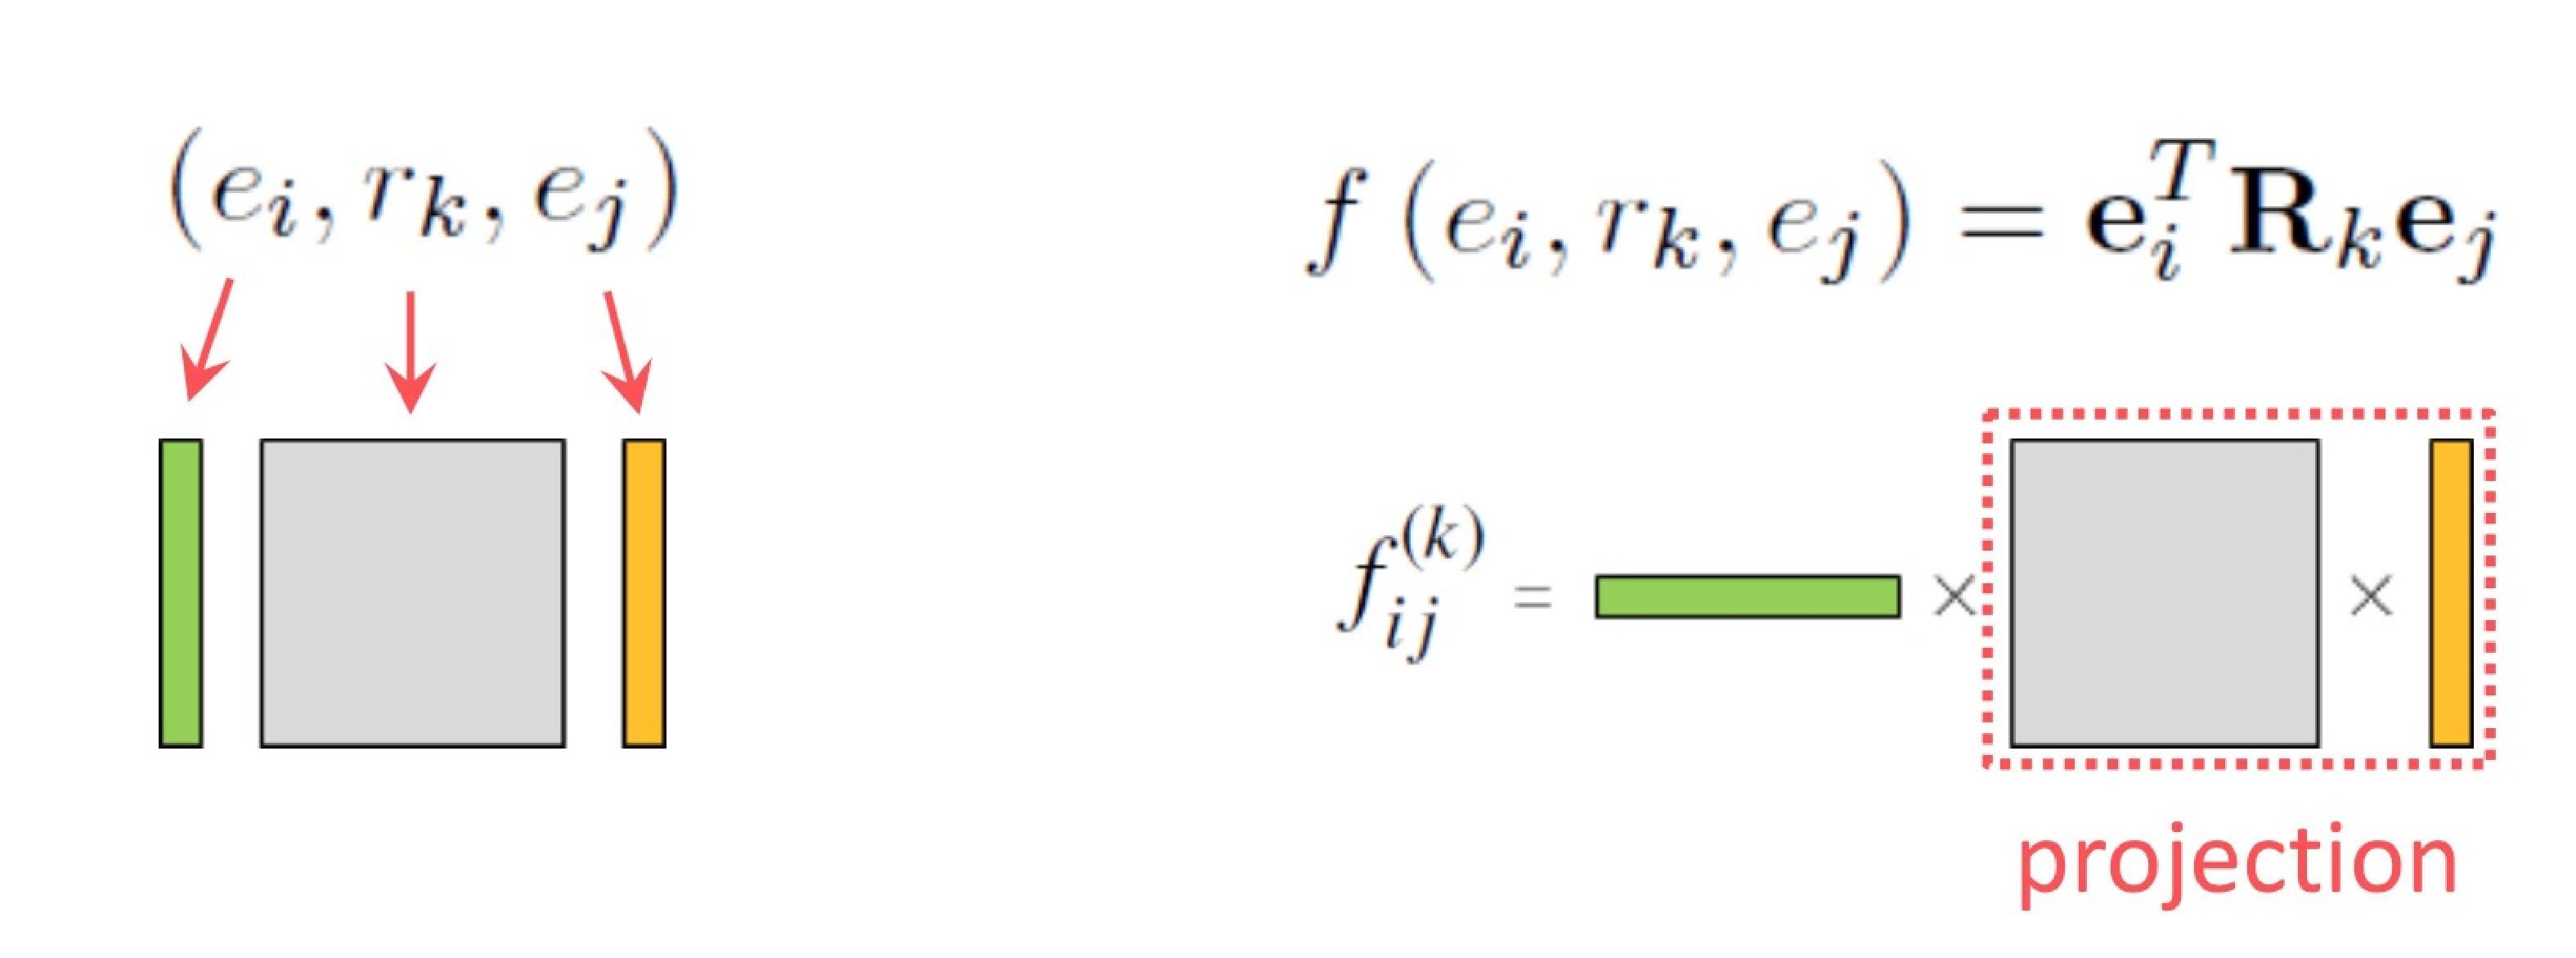
\includegraphics[width=0.90\textwidth,height=0.30\textwidth]{5.eps}
		\end{figure}
	\item Learn based on reconstruction error:
		\begin{equation}
			\min_{e_i,R_k}\sum_k\sum_i\sum_j{(y_{i,j}^k-f(e_i,r_k,e_j))^2+\lambda R}
		\end{equation}
	\begin{exampleblock}{assumption}
		It is assumed that all pairs not contained in dataset are negative.
	\end{exampleblock}
\end{itemize}
\end{frame}

\subsection{Methods based on ranking loss}
\begin{frame}
\frametitle{NTN: ranking loss}
\begin{itemize}
	\item Representation in hidden vector/matrix space and the corresponding fitness function:
		\begin{figure}
			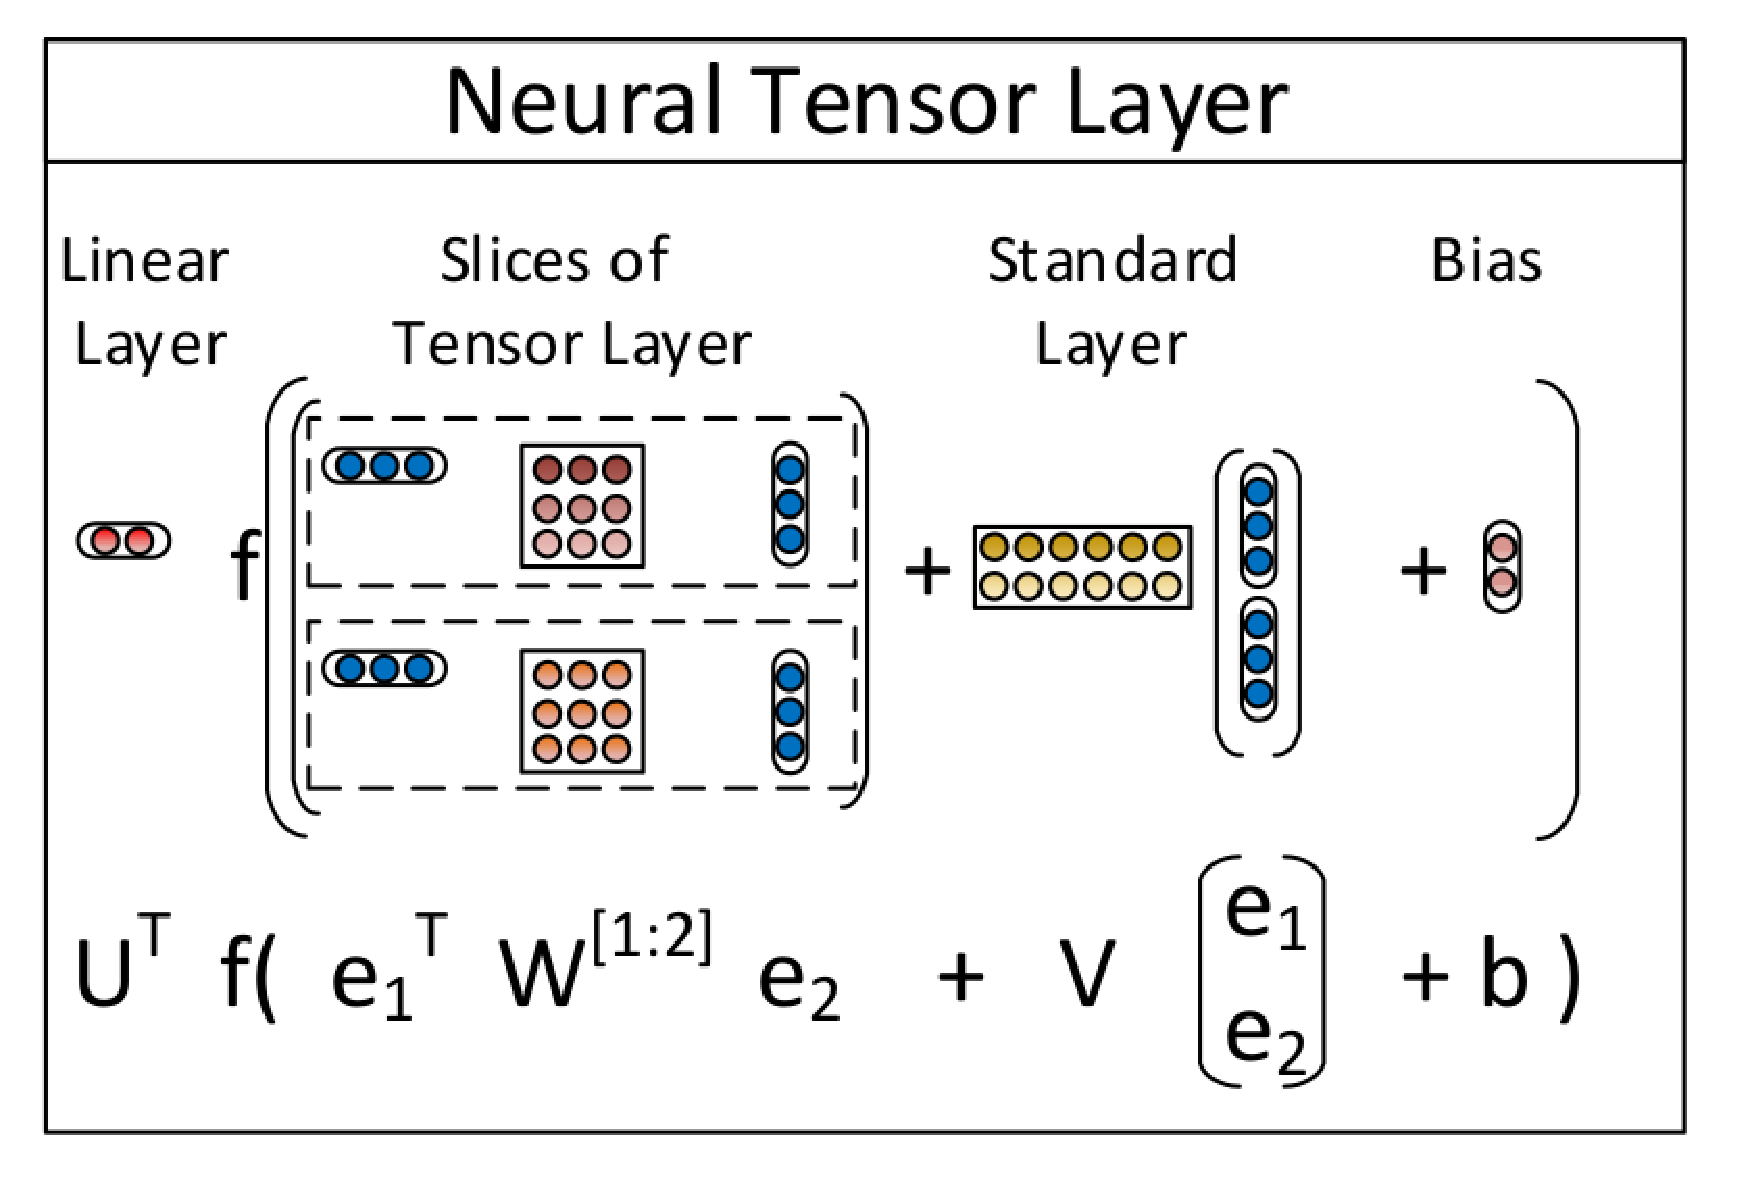
\includegraphics[width=0.60\textwidth,height=0.30\textwidth]{7.eps}
		\end{figure}
		\begin{equation}
			f(e_i,r_k,e_j)=U_k^Tg(e_i^TW_k^{[1:K]}e_j + V_k[e_i:e_j] + b_k)
		\end{equation}
	\item Learn based on reconstruction error:
		\begin{equation}
			\min_{e_i,R_k}\sum_{t^+ \in O}\sum_{t^- \in D}{(\lambda + f(e_i,r_k,e_j) - f(e'_i,r_k,e'_j))}
		\end{equation}
	\begin{exampleblock}{assumption}
		It is assumed that all pairs not contained in dataset are negative.
	\end{exampleblock}
\end{itemize}
\end{frame}

\begin{frame}
\frametitle{TransE: ranking loss}
\begin{itemize}
	\item Representation in hidden vector space and the corresponding fitness function:
		\begin{figure}
			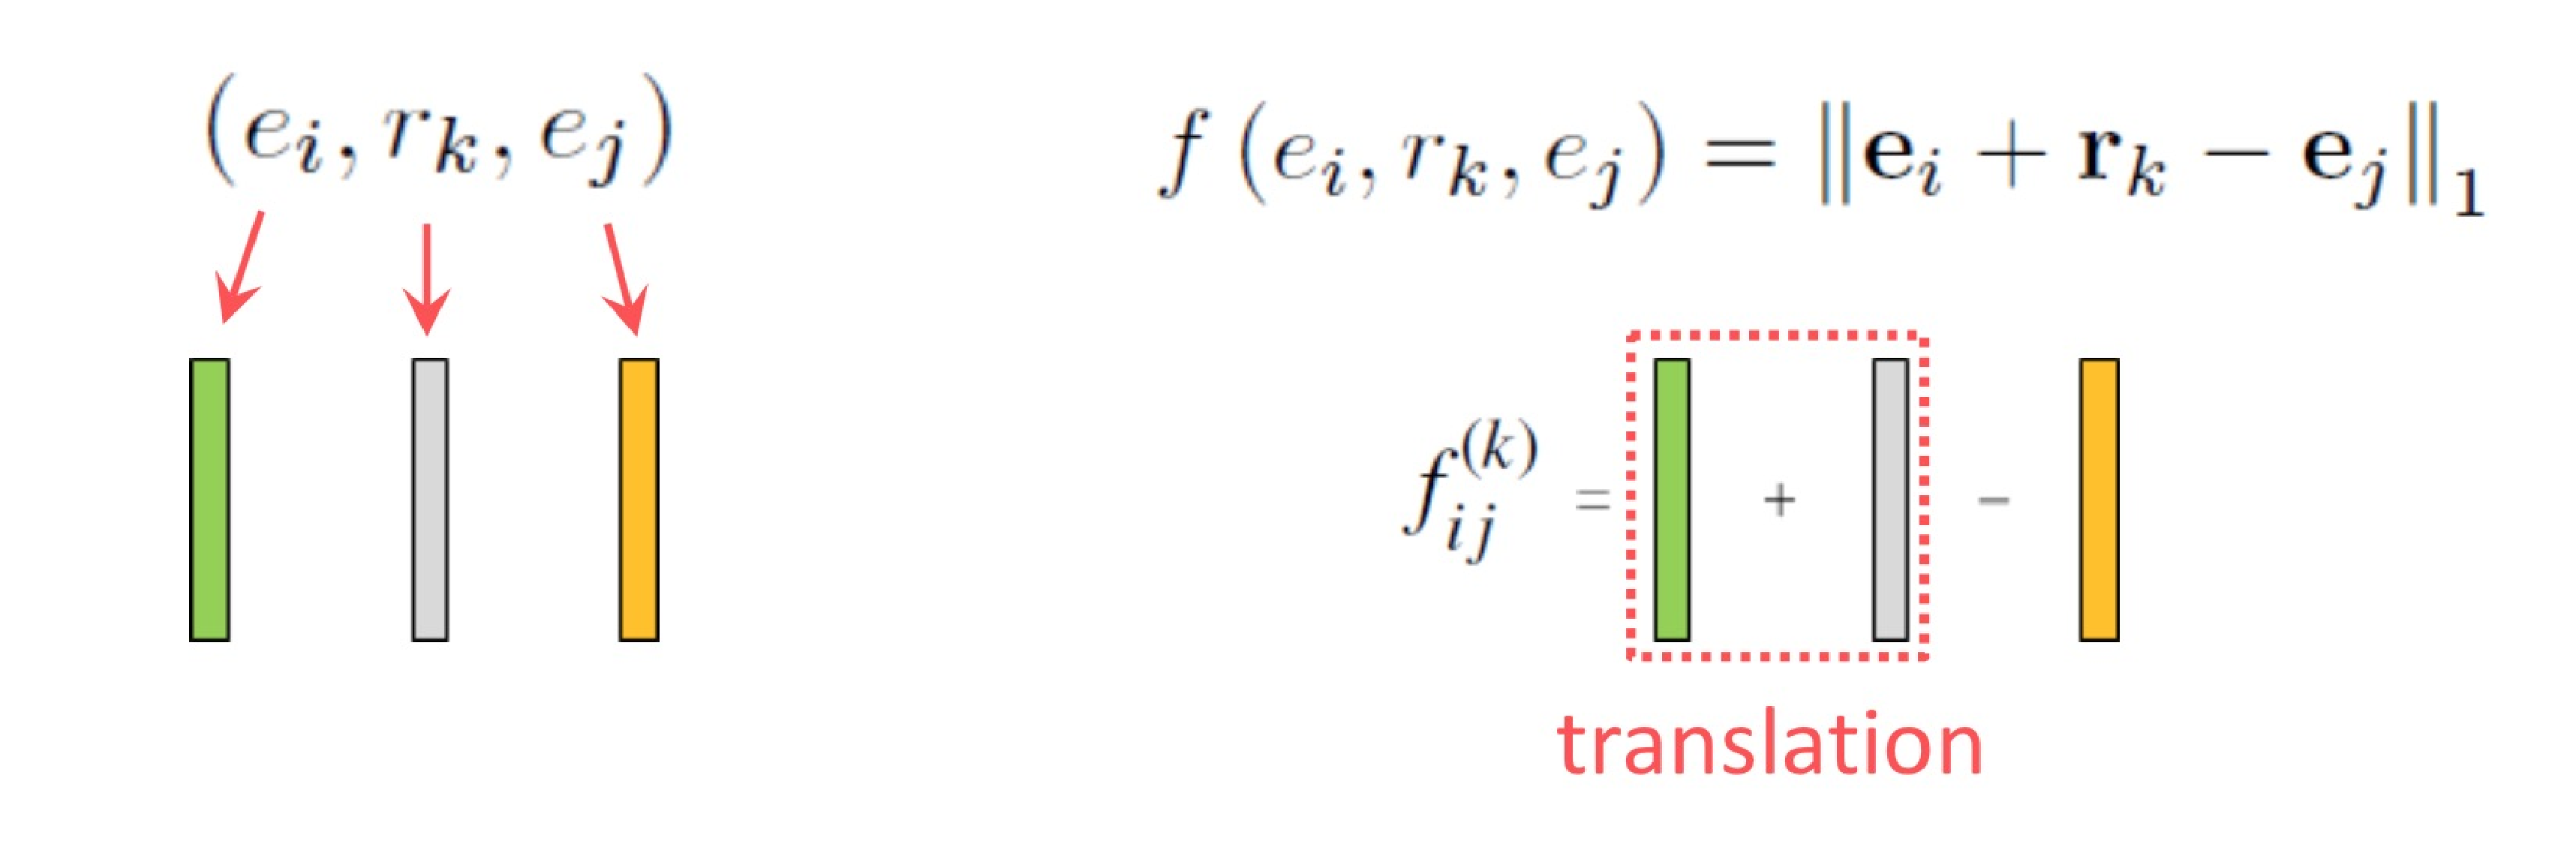
\includegraphics[width=0.90\textwidth,height=0.30\textwidth]{6.eps}
		\end{figure}
	\item Learn based on ranking loss:
		\begin{equation}
			\min_{e_i,R_k}\sum_{t^+ \in O}\sum_{t^- \in D}{(\lambda + f(e_i,r_k,e_j) - f(e'_i,r_k,e'_j))}
		\end{equation}
	\begin{exampleblock}{assumption}
		It is assumed that pairs not contained in dataset are partially negative.
	\end{exampleblock}
\end{itemize}
\end{frame}

\subsection{Pros and Cons}
\begin{frame}
\frametitle{Prons and Cons}
\begin{itemize}
	\item Pros
		\begin{enumerate}
			\item Hidden space model can capture the complex concepts.
			\item It is computationally efficient.
		\end{enumerate}
	\item Cons
		\begin{enumerate}
			\item It is not logical: we can capture the co-occurrence information but not logical properties of relation.
			\item It is not precise: data-driven methods will be noisy-prone.
		\end{enumerate}
\end{itemize}
\end{frame}


\bibliography{ref}
\end{document}
